\textbf{{定点数的移位运算}}

\textbf{(1)逻辑移位}

逻辑移位规则:逻辑左移时,高位移丢,低位补0;逻辑右移时,低位移丢,高位添0,例如,寄存器的内容为10001010,逻辑左移为00010100,逻辑右移为01000101。

\textbf{(2)算术移位}

算术移位规则总结如下表:

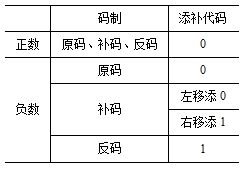
\includegraphics[width=2.55208in,height=1.77083in]{png-jpeg-pics/6702B9B4984FC8F172C1A131535E1BB7.png}

{\textbf{原码定点数的加}}{\textbf{/}}{\textbf{减运算}}

{{\textbf{1)加法规则:}先判断符号位,若相同,绝对值相加,结果符号位不变;若不同,则做减法,绝对值大的数减去绝对值小的数,结果符号与绝对值大的数相同。}}

{\textbf{2)减法规则:}两个原码表示的数相减,首先将减数符号取反,然后将被减数与符号取反后的减数按原码加法进行运算。}

{{\textbf{补码定点数的加/减运算}}{\textbf{}}\\
}

{{\textbf{{(1)补码加法}}}}

{两个数的补码相加,符号位参加运算,且两数和的补码等于两数的补码之和,公式是如下:}

{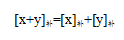
\includegraphics[width=1.29167in,height=0.41667in]{png-jpeg-pics/3F34CD6B8EAA9A7F1C52ECACA7825AF7.png}\\
}

\textbf{(2)补码减法}

\textbf{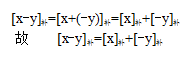
\includegraphics[width=1.97917in,height=0.60417in]{png-jpeg-pics/4CCA533CE368F5FECF12C90D5D4DA66C.png}\\
}

\textbf{{溢出的概念和判别方法}}

\textbf{(1)溢出产生的原因}

\textbf{溢出的概念:}假设机器字长固定,不妨设为8位(包含一位符号位),根据前面掌握的知识,补码的取值范围应该是-128~127,若现在两个数相加大于127,或者小于-128,则称为溢出,其中两数相加大于上界127,称为上溢或者正溢出;两数相加小于下界-128,称为下溢或者负溢出。定点小数的情况相同,若两个定点小数相加大于或等于1,则称为上溢;若两个定点小数相加小于-1,则称为下溢。

\textbf{(2)计算机是怎么判断溢出的呢?一共有以下3种方法。}

\textbf{1)方法一:从两个数的符号位出发。}

讲解之前先介绍两个必须知道的概念:

\textbf{①
对于加法,}只有在正数加正数或负数加负数两种情况下才有可能出现溢出,符号不同的两个数相加是不会溢出的。

\textbf{②
对于减法,}只有在正数减负数或负数减正数两种情况下才有可能出现溢出,符号相同的两个数相减是不会溢出的。

由于减法运算在机器中是用加法器实现的,因此可得出如下结论:不论是做加法,还是做减法,只要实际参加操作的两个数(减法时即为被减数和``求补''以后的减数)符号相同,结果又与原操作数的符号不同,即认为溢出。

\textbf{2)方法二:仍然是从两个数的符号位出发。}

在计算机中,一般都是通过数值部分最高位的进位(或者称为最高有效位)和符号位产生的进位进行``异或''操作,然后按照``异或''的结果进行判断(``异或''就是两数不同时为1,两数相同时为0)。若``异或''结果为1,则为溢出;若``异或''结果为0,则无溢出。

\textbf{3)方法三:用两位符号位判断溢出。}

\textbf{变形补码判断溢出的原则:}当两位符号位不同时,表示溢出,否则,无溢出。无论是否发生溢出,高位符号位永远代表真正的符号位。再深入分析一下:假设现在运算结果的符号位为01,而高位符号代表的是真正的符号位,可以判断这个结果一定是一个正数,既然是正数则肯定是正溢出;反之,运算结果的符号位是10,则是负溢出。

{定点数的乘除法内容较多,不适合手机观看,详见《计算机组成原理高分笔记》。}
